\documentclass[12pt]{article}
\usepackage[utf8]{inputenc}
\usepackage[spanish]{babel}
\usepackage{bbding}
\decimalpoint
\usepackage[spanish]{babel}
\usepackage{amsmath}
\usepackage{amsthm}
\usepackage{amssymb}
\usepackage{graphicx}
\usepackage[margin=0.9in]{geometry}
\usepackage{fancyhdr}
\usepackage[inline]{enumitem}
\usepackage{float}
\usepackage{cancel}
\usepackage{minted}
\usepackage{bigints}
\usepackage{color}
\usepackage{xcolor}
\usepackage{subfig}
\usepackage{listingsutf8}
\usepackage{algorithm}
\usepackage{tocloft}
\usepackage[none]{hyphenat}
\usepackage{graphicx}
\usepackage{grffile}
\usepackage{tabularx}
\usepackage[nottoc,notlot,notlof]{tocbibind}
\usepackage{times}
\usepackage{color}
\definecolor{gray97}{gray}{.97}
\definecolor{gray75}{gray}{.75}
\definecolor{gray45}{gray}{.45}
\renewcommand{\cftsecleader}{\cftdotfill{\cftdotsep}}
\pagestyle{fancy}
\setlength{\headheight}{15pt} 
\lhead{Práctica 6 - Comunicación inter procesos (IPC) en Linux y Windows}
\rhead{\thepage}
\lfoot{ESCOM-IPN}
\renewcommand{\footrulewidth}{0.5pt}
\setlength{\parskip}{0.5em}
\newcommand{\ve}[1]{\overrightarrow{#1}}
\newcommand{\abs}[1]{\left\lvert #1 \right\lvert}
\date{26 de febrero de 2017}
\title{Instalación de Netbeans}
\author{Reporte 1}

\definecolor{pblue}{rgb}{0.13,0.13,1}
\definecolor{pgreen}{rgb}{0,0.5,0}
\definecolor{pred}{rgb}{0.9,0,0}
\definecolor{pgrey}{rgb}{0.46,0.45,0.48}
\lstset{tabsize=1}

\usepackage{listings}
\lstset{ frame=Ltb,
framerule=0pt,
aboveskip=0.5cm,
framextopmargin=3pt,
framexbottommargin=3pt,
framexleftmargin=0.4cm,
framesep=0pt,
rulesep=.4pt,
backgroundcolor=\color{gray97},
rulesepcolor=\color{black},
%
stringstyle=\ttfamily,
showstringspaces = false,
basicstyle=\small\ttfamily,
commentstyle=\color{gray45},
keywordstyle=\bfseries,
%
numbers=left,
numbersep=15pt,
numberstyle=\tiny,
numberfirstline = false,
breaklines=true,
}

% minimizar fragmentado de listados
\lstnewenvironment{listing}[1][]
{\lstset{#1}\pagebreak[0]}{\pagebreak[0]}

\lstdefinestyle{consola}
{basicstyle=\scriptsize\bf\ttfamily,
backgroundcolor=\color{gray75},
}

\lstdefinestyle{C}
{language=C,
}
 \lstset{style=CompilandoStyle}                                  %Use this style

    \usepackage{minted} % Paquete que permite citar codigo
    \usemintedstyle{borland} % Aqui se define el colorscheme para minted
    \setminted{
        fontsize = \scriptsize, % Ajusta el codigo a la hoja
        baselinestretch = 1,
        linenos, % set numbers
        breaklines=true, % Hace un salto de linea automatico en caso de que se llege al final de la line
        tabsize=3 
    }
%%%%%%%%%%%%%%%%%%%%%

\lstdefinestyle{customc}{
  belowcaptionskip=1\baselineskip,
  breaklines=true,
  frame=L,
  xleftmargin=\parindent,
  language=C,
  showstringspaces=false,
  basicstyle=\footnotesize\ttfamily,
  keywordstyle=\bfseries\color{green!40!black},
  commentstyle=\itshape\color{purple!40!black},
  identifierstyle=\color{blue},
  stringstyle=\color{orange},
}

\lstdefinestyle{customasm}{
  belowcaptionskip=1\baselineskip,
  frame=L,
  xleftmargin=\parindent,
  language=[x86masm]Assembler,
  basicstyle=\footnotesize\ttfamily,
  commentstyle=\itshape\color{purple!40!black},
}

\lstset{escapechar=@,style=customc}

    % =====  CODE EDITOR =========
    \lstdefinestyle{CompilandoStyle} {                              %This is Code Style
        backgroundcolor=\color{BlueGrey800MD},                      %Background Color  
        basicstyle=\tiny\color{white},                              %Font color
        commentstyle=\color{BlueGrey100MD},                         %Comment color
        stringstyle=\color{TealMD},                                 %String color
        keywordstyle=\color{Green100MD},                            %keywords color
        numberstyle=\tiny\color{TealMD},                            %Size of a number
        frame=shadowbox,                                            %Adds a frame around the code
        breakatwhitespace=true,                                     %Style                       
        breaklines=true,                                            %Style                   
        keepspaces=true,                                            %Style                   
        numbers=left,                                               %Style                   
        numbersep=10pt,                                             %Style 
        xleftmargin=\parindent,                                     %Style 
        tabsize=4                                                   %Style 
    }
 
    \lstset{style=CompilandoStyle}                                  %Use this style

    \usepackage{minted} % Paquete que permite citar codigo
    \usemintedstyle{borland} % Aqui se define el colorscheme para minted
    \setminted{
        fontsize = \scriptsize, % Ajusta el codigo a la hoja
        baselinestretch = 1,
        linenos, % set numbers
        breaklines=true, % Hace un salto de linea automatico en caso de que se llege al final de la line
        tabsize=3 
    }


%Permite crear columnas en el documento
\usepackage{multicol} 
\usepackage{color}
\usepackage{comment}
\newcommand{\tabitem}{~~\llap{\textbullet}~~}
\newcommand{\subtabitem}{~~~~\llap{\textbullet}~~}

\usepackage{cmbright}                               % Font


\bibliographystyle{IEEEtran}
\begin{document}
    \begin{titlepage}
      \begin{center}
        
        % Upper part of the page. The '~' is needed because \\
        % only works if a paragraph has started.
        
        \noindent
        \begin{minipage}{0.5\textwidth}
          \begin{flushleft} \large
            \includegraphics[width=0.3\textwidth]{../ipn.png}
          \end{flushleft}
        \end{minipage}%
        \begin{minipage}{0.55\textwidth}
          \begin{flushright} \large
            \includegraphics[width=0.7\textwidth]{../escom.png}
          \end{flushright}
        \end{minipage}
        
        \textsc{\LARGE Instituto Politécnico Nacional}\\[0.5cm]
        
        \textsc{\Large Escuela Superior de Cómputo}\\[1cm]
        
        % Title
        
        { \huge Práctica 6 - Comunicación inter procesos (IPC) en Linux y Windows \\[1cm] }
        
        { \Large Unidad de aprendizaje: Sistemas Operativos} \\[1cm]
        
        { \Large Grupo: 2CM8 } \\[1cm]
        
        \noindent
        \begin{minipage}{0.5\textwidth}
          \begin{flushleft} \large
            \emph{Alumnos(a):}\\
            
            \begin{tabular}{ll}
             Briones Tapia Mariana \\
             Méndez Mejía Sergio Ernesto \\
             Nicolás Sayago Abigail\\
             Ramos Diaz Enrique \\
               
          \end{tabular}
          \end{flushleft}
        \end{minipage}%
        \begin{minipage}{0.5\textwidth}
          \begin{flushright} \large
            \emph{Profesor(a):} \\
            Cortes Galicia Jorge  \\
          \end{flushright}
        \end{minipage}
        
        \vfill
        
        % Bottom of the page
        {\large 26 de noviembre 2018}
      \end{center}
    \end{titlepage}
  
  \tableofcontents
  \newpage
  
  
  % ////////////////////////////////////////////////////////////////////////////////////
  %                                    COMPETENCIAS
  % ////////////////////////////////////////////////////////////////////////////////////

  \section{Competencias}
  El alumno comprende el funcionamiento de las tuberías (pipes) sin nombre y de la memoria compartida como mecanismos de comunicación entre procesos tanto en el sistema operativo Linux como Windows para el desarrollo de aplicaciones concurrentes con soporte de comunicación.
  \begin{itemize}
      \item Revisión de tuberías y memoria compartida tanto en Linux como en Windows.
        \item Revisión de las llamadas al sistema para tuberías y memoria compartida en ambos sistemas operativos.
        \item Desarrollo de aplicaciones concurrentes que requieren comunicación en Linux y Windows.
  \end{itemize}

  % ////////////////////////////////////////////////////////////////////////////////////
  %                                     DESARROLLO
  % ////////////////////////////////////////////////////////////////////////////////////

  \section{Desarrollo}

    % //////////////////////////////////////////////////////////////////////////////////
    %                      Puntos a observar y reportar
    % /////////////////////////////////////////////////////////////////////////////////
  
    \subsection{Puntos a observar y reportar}
              
      % /////////////////////////////////////////////////////////////////////
      %                              SECCION DE LINUX
      % /////////////////////////////////////////////////////////////////////
                
      \subsubsection{Sección Linux:}
      Investigación de los siguientes comandos:

      \begin{itemize}
        \item[\Checkmark] \textbf{pipe()} \\

            \begin{figure}[h!]
                \centering
               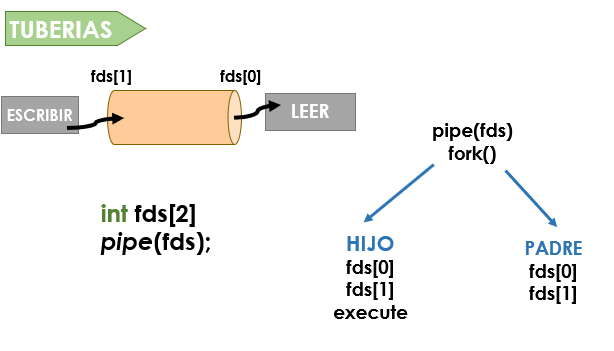
\includegraphics[width=0.9\textwidth]{Practica6/Images/General/Tuberias.PNG}
            \end{figure}
            Permite enviar la salida de uno comando a otro. Una \textsf{tubería}, como suele decirse, puede redirigir la salida estándar, la entrada o el error de un proceso a otro para su posterior procesamiento.

            La sintaxis para el comando es con el carácter $|$ entre dos comandos:
    
            \begin{figure}[h!]
                    \centering
                   
\includegraphics[width=0.7\textwidth]{Practica6/Images/General/Comandos.PNG}
            \end{figure}
    
            No se puede acceder a la tubería a través de otra sesión, se crea temporalmente para acomodar la ejecución del \textbf{Comando 1} y redirigir la salida estándar. Se elimina después de la ejecución exitosa.
    
            Una tubería con nombre puede durar hasta que el sistema esté en funcionamiento o hasta que se elimine. Es un archivo especial que sigue el mecanismo \textbf{FIFO} $($ Primero en entrar, primero en salir$)$. Se puede utilizar como un archivo normal, es decir, puede escribir, leer, abrir o cerrar. Para crear una tubería con nombre se usa el comando:
    
            \begin{figure}[h!]
                    \centering
                   
\includegraphics[width=0.4\textwidth]{Practica6/Images/General/mkfifo.PNG}
            \end{figure}

        \item[\Checkmark] \textbf{shmget()}
            
            Asigna un segmento de memoria compartida de System V. Retorna el identificador del segmento de memoria compartida de System V asociado con el valor del argumento \textbf{key}. Puede ser usado ya sea para obtener el identificador de un segmento de memoria compartida creada previamente $($ cuando shmglh es cero y la clave no tiene valorIPC$_$PRIVATE $)$, o para crear un nuevo conjunto.
            
            Un nuevo segmento de memoria compartida, con tamaño igual que el valor de \textbf{size} redondeado a un múltiplo de \textbf{PAGE$_$SIZE}, se crea si la clave tiene el valor \textbf{IPC$_$PRIVATE}.
        
            % DE: http://man7.org/linux/man-pages/man2/shmget.2.html
        
        \item[\Checkmark] \textbf{shmat()}
            Adjunta el segmento de memoria compartida asociado con el identificador de memoria compartida especificado por shmid al espacio de direcciones del proceso de llamado.
            
            % DE: http://pubs.opengroup.org/onlinepubs/009604599/functions/shmat.html
      \end{itemize}
      
          
        \begin{itemize}
            \item[\Checkmark] \textbf{Punto 2: Tuberías en Linux} 
            \begin{multicols}{2}
                \inputminted{c++}{Code/Linux/2.c}
            \end{multicols}
                
            \item[\Checkmark] \textbf{Punto 5: Memoria compartida en Linux} 
            
                 CLIENTE: 
                \inputminted{c++}{Code/Linux/5_cliente.c}
                SERVIDOR:
                \inputminted{c++}{Code/Linux/5_servidor.c}
                
        \end{itemize}
        
      
      % /////////////////////////////////////////////////////////////////////
      %                              SECCION DE WINDOWS
      % /////////////////////////////////////////////////////////////////////
          
      \subsubsection{Sección Windows:}
            \begin{itemize}
                \item[\Checkmark] \textbf{Punto 3: Tuberías en Windows} 
                \inputminted{c++}{Code/Windows/3.c}
               
                PROGRAMA HIJO
                 \inputminted{c++}{Code/Windows/3_hijo.c}

                \item[\Checkmark] \textbf{Punto 6: Memoria compartida en Windows} 
               
               CLIENTE \inputminted{c++}{Code/Windows/6_cliente.c}
               
               SERVIDOR \inputminted{c++}{Code/Windows/6_servidor.c}
            \end{itemize}

                   
    % //////////////////////////////////////////////////////////////////////////////////
    %                   CODIGOS FUENTE DE LOS PROGRAMAS DESARROLLADOS
    % /////////////////////////////////////////////////////////////////////////////////

    \subsection{Explicación general de los programas}
        \begin{figure}[h!]
                \centering
               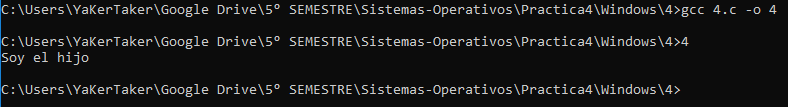
\includegraphics[width=1.0\textwidth]{Practica6/Images/General/4.PNG}
        \end{figure}

    \subsection{Códigos fuente de los programas desarrollados}
    
      % /////////////////////////////////////////////////////////////////////
      %                              SECCION DE LINUX
      % /////////////////////////////////////////////////////////////////////

      \subsubsection{Sección Linux}
      \begin{itemize}
        \item [\Checkmark]\textbf{Punto 4: Inversa de la suma y multiplicación de matrices con tuberías}
          \inputminted{c++}{Code/Linux/4.c}
        \item[\Checkmark] \textbf{Punto 7: Inversa de la suma y multiplicación de matrices con memoria compartida}
          \inputminted{c++}{Code/Linux/7.c}
      \end{itemize}


      % /////////////////////////////////////////////////////////////////////
      %                              SECCION DE WINDOWS
      % /////////////////////////////////////////////////////////////////////
    
      \subsubsection{Sección Windows}
      \begin{itemize}
        \item [\Checkmark]\textbf{Punto 4: Inversa de la suma y multiplicación de matrices con tuberías}
          \inputminted{c++}{Code/Windows/4.c}
        
        \item[\Checkmark] \textbf{Punto 7: Inversa de la suma y multiplicación de matrices con memoria compartida}
        
            PROGRAMA ABUELO: Envía 2 matrices a multiplicar, recibe suma y multiplicación, guarda sus inversas en archivos.
            
            \inputminted{c++}{Code/Windows/7_1.c}
            
            PROGRAMA PADRE: Envía 2 matrices a sumar, multiplica matrices recibidas del abuelo y la envía al abuelo.
            
            \inputminted{c++}{Code/Windows/7_2.c}
            
            PROGRAMA HIJO: Recibe 2 matrices a sumar, las suma y envía al abuelo.
              \inputminted{c++}{Code/Windows/7_3.c}
      \end{itemize}
        
\newpage

    % ////////////////////////////////////////////////////////////////////////////////////////////////////
    %                      PANTALLAS DE EJECUCIÓN DE LOS PROGRAMAS DESARROLLADOS
    % ////////////////////////////////////////////////////////////////////////////////////////////////////      

    \subsection{Pantallas de ejecución de los programas desarrollados}
          
      % /////////////////////////////////////////////////////////////////////
      %                              SECCION DE LINUX
      % /////////////////////////////////////////////////////////////////////
        
      \subsubsection{Sección Linux:}
      \begin{itemize}
      
          \item[\Checkmark] \textbf{Punto 2: Tuberías en Linux} 
                \begin{figure}[h!]
                        \centering
                       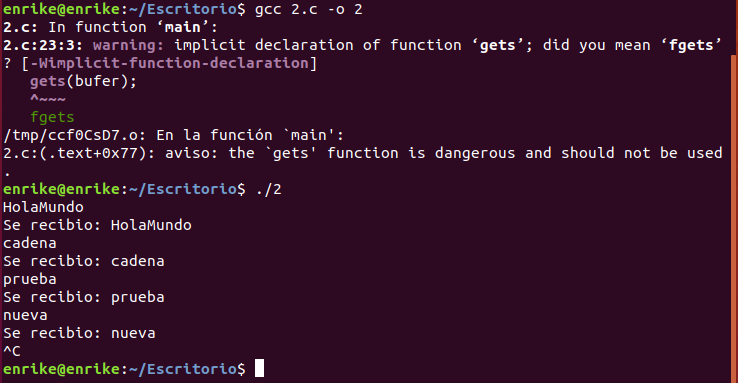
\includegraphics[width=0.73\textwidth]{Practica6/Images/Linux/2.png}
                \end{figure}

            \item[\Checkmark]{\textbf{Punto 4: Multiplicación e inversa de matrices con Tuberías}}
                
          \begin{figure}[h!]
              \centering
            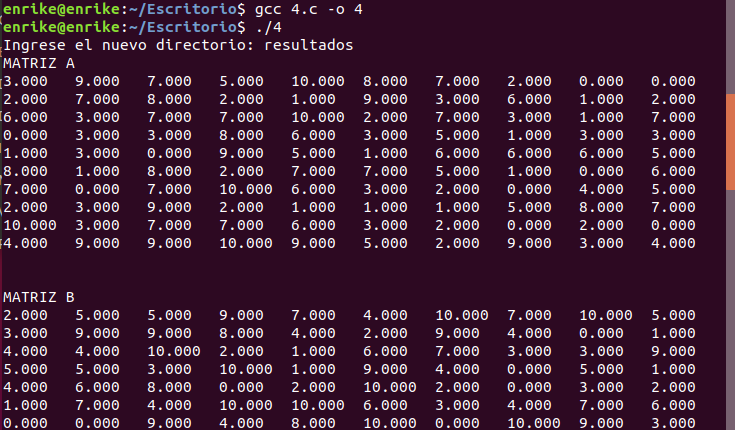
\includegraphics[width=0.73\textwidth]{Practica6/Images/Linux/4_1.png}
              
          \end{figure}
\newpage
          \begin{figure}[h!]
              \centering  
            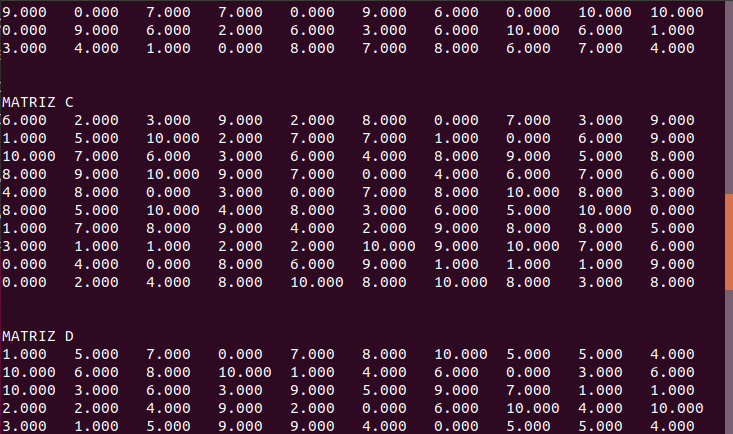
\includegraphics[width=0.73\textwidth]{Practica6/Images/Linux/4_2.png}  
            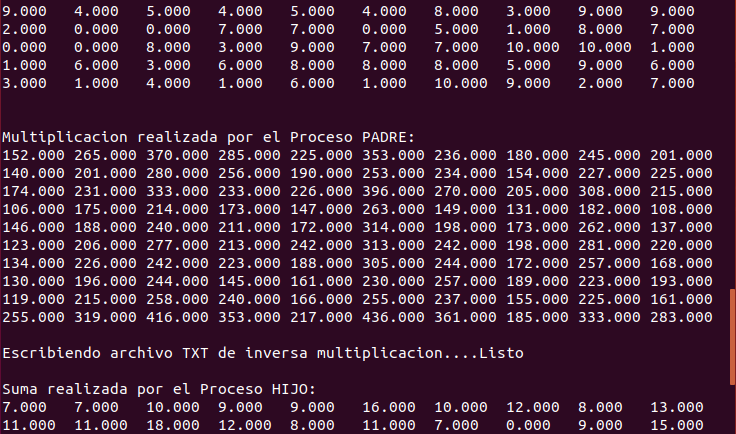
\includegraphics[width=0.73\textwidth]{Practica6/Images/Linux/4_3.png}
            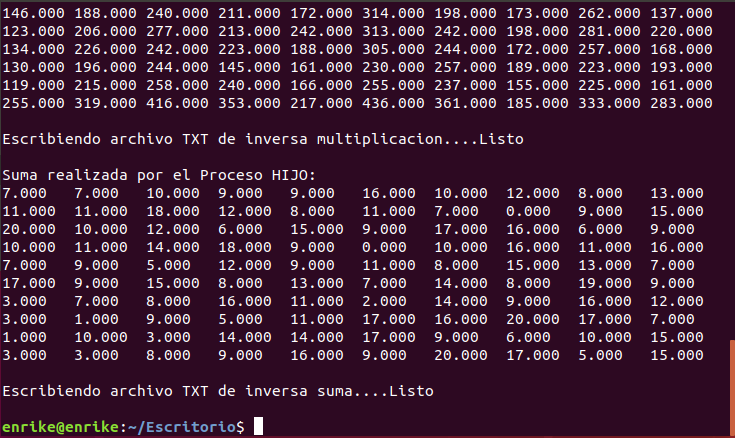
\includegraphics[width=0.73\textwidth]{Practica6/Images/Linux/4_4.png}
            
          \end{figure}
      
      \clearpage
          \begin{figure}[h!]
              \centering  
              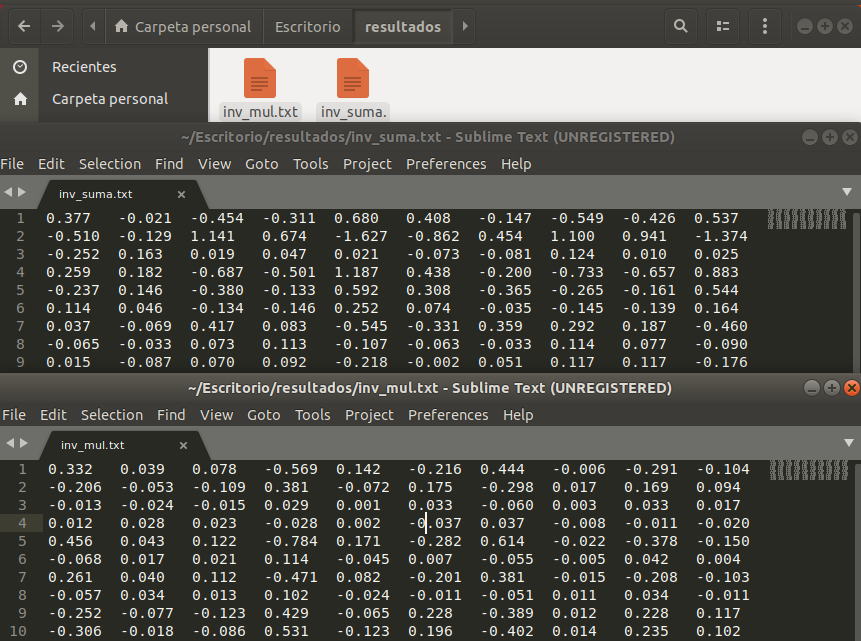
\includegraphics[width=0.71\textwidth]{Practica6/Images/Linux/4_5.png}
            
          \end{figure}

            \item[\Checkmark] \textbf{Punto 5: Memoria compartida en Linux} 
                \begin{figure}[h!]
                        \centering
                       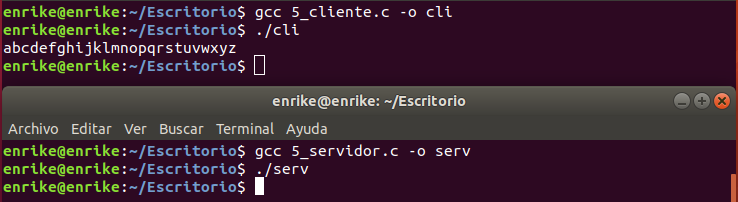
\includegraphics[width=0.73\textwidth]{Practica6/Images/Linux/5.png}
                \end{figure}

            \item[\Checkmark] \textbf{Punto 7: Inversa de la suma y multiplicación de matrices con memoria compartida} 
                 \begin{figure}[h!]
                        \centering
                       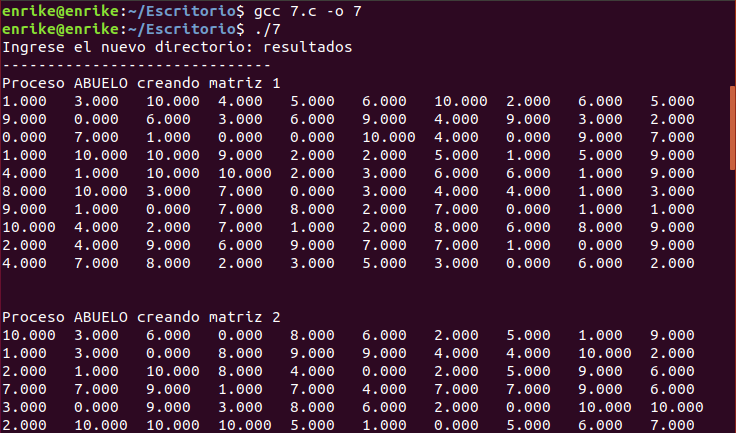
\includegraphics[width=0.73\textwidth]{Practica6/Images/Linux/7_1.png}
                \end{figure}
                \begin{figure}[h!]
                        \centering
                       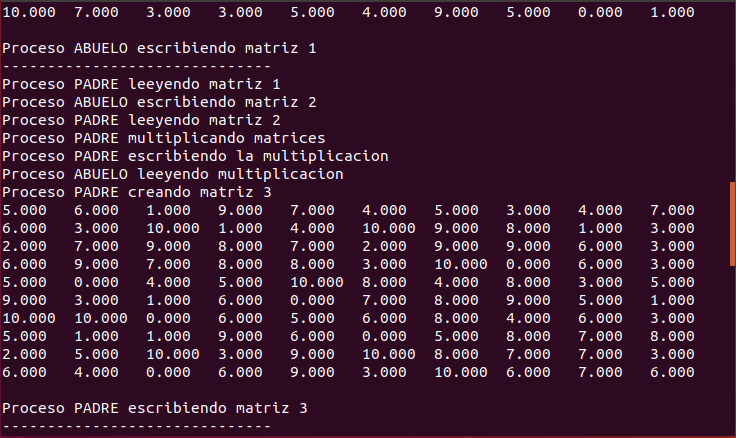
\includegraphics[width=0.73\textwidth]{Practica6/Images/Linux/7_2.png}
                       
                       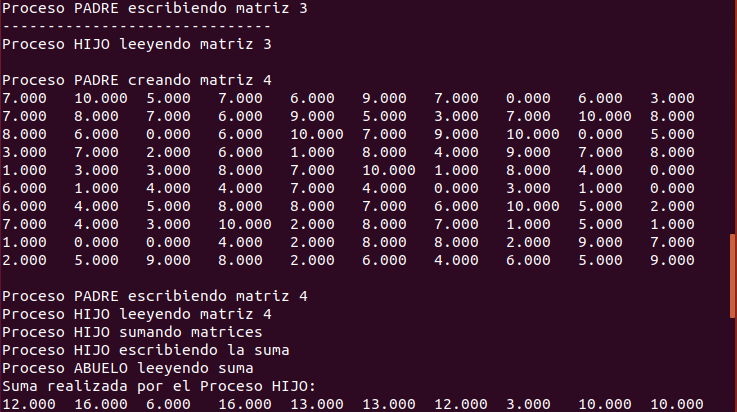
\includegraphics[width=0.73\textwidth]{Practica6/Images/Linux/7_3.png}
                       
                       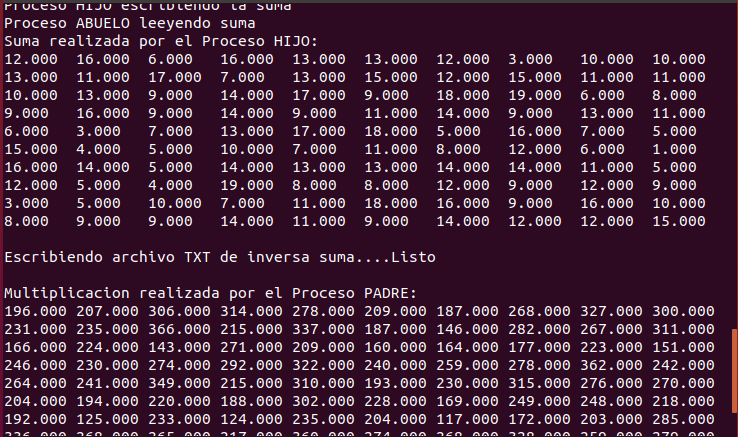
\includegraphics[width=0.73\textwidth]{Practica6/Images/Linux/7_4.png}
                       
                \end{figure}
            \clearpage
                \begin{figure}[h!]
                        \centering
                         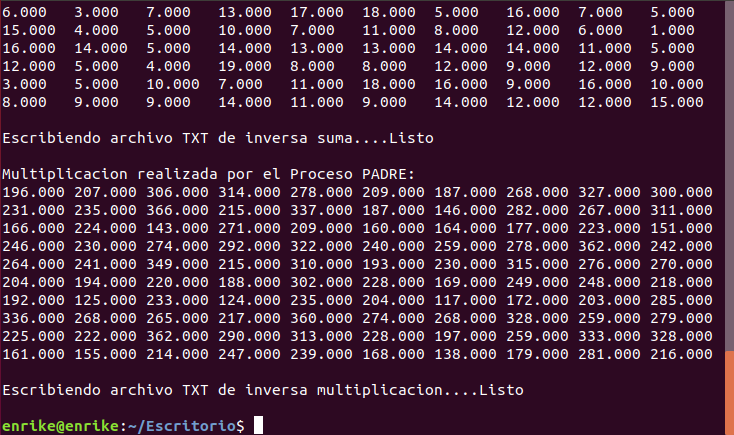
\includegraphics[width=0.73\textwidth]{Practica6/Images/Linux/7_5.png}
                       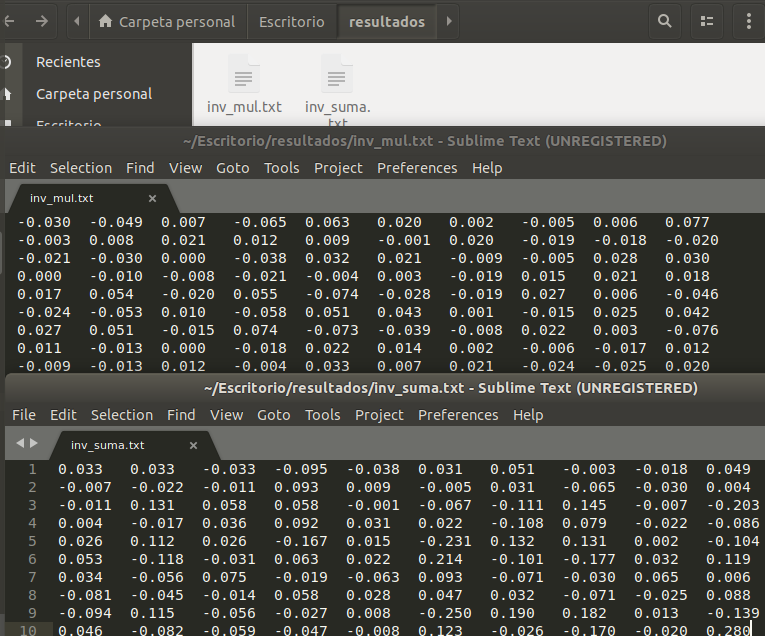
\includegraphics[width=0.73\textwidth]{Practica6/Images/Linux/7_6.png}
                       
                \end{figure}
        \end{itemize}
                   
      % /////////////////////////////////////////////////////////////////////
      %                              SECCION DE WINDOWS
      % /////////////////////////////////////////////////////////////////////
        
      \subsubsection{Sección Windows:}
      \begin{itemize}
      
          \item[\Checkmark] \textbf{Punto 3: Tuberías en Windows} 
                \begin{figure}[h!]
                        \centering
                       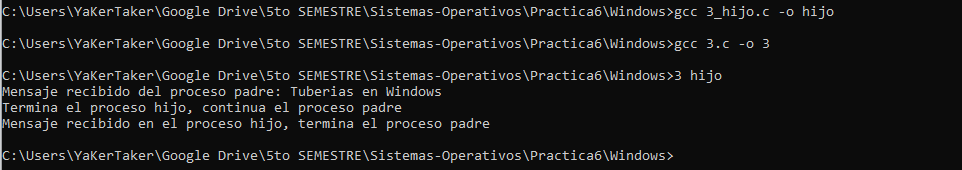
\includegraphics[width=0.8\textwidth]{Practica6/Images/Windows/3.PNG}
                \end{figure}
            \newpage
            \item[\Checkmark] \textbf{Punto 4: Multiplicación e inversa de matrices con Tuberías} 
                \begin{figure}[h!]
                        \centering
                       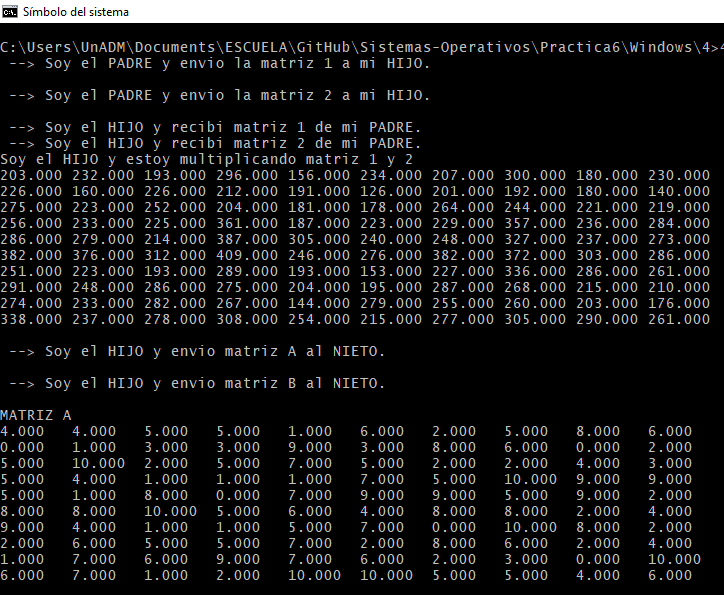
\includegraphics[width=0.76\textwidth]{Practica6/Images/Windows/4/4_1.PNG}
                       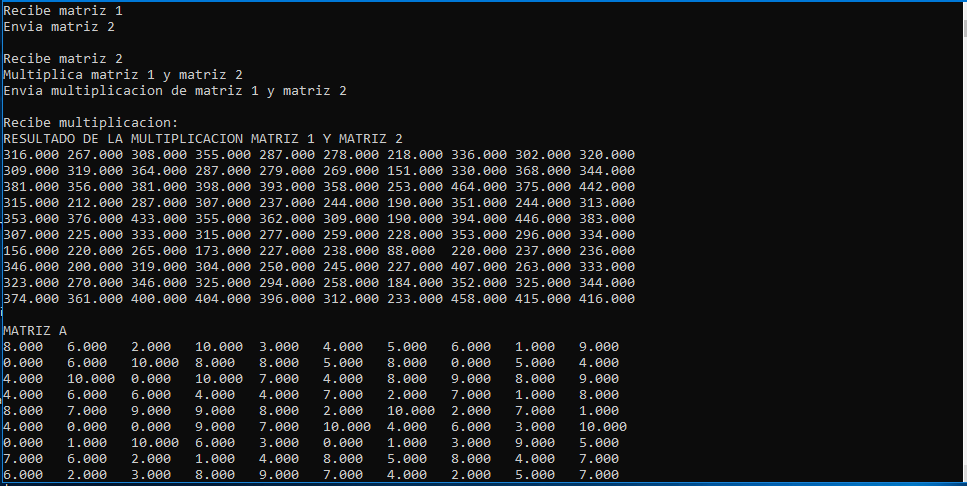
\includegraphics[width=0.76\textwidth]{Practica6/Images/Windows/4/4_2.PNG}
                \end{figure}
                 \begin{figure}[h!]
                        \centering
                       
                       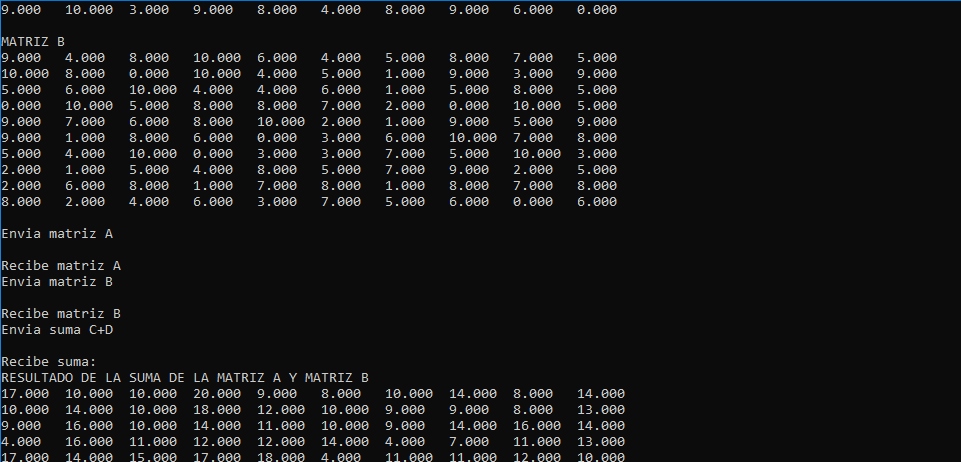
\includegraphics[width=0.82\textwidth]{Practica6/Images/Windows/4/4_3.PNG}
                       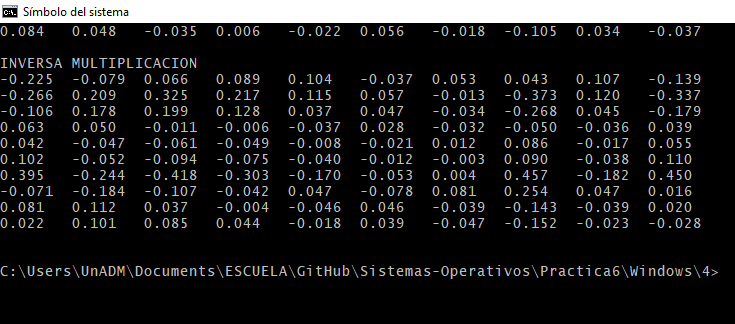
\includegraphics[width=0.82\textwidth]{Practica6/Images/Windows/4/4_4.PNG}
                       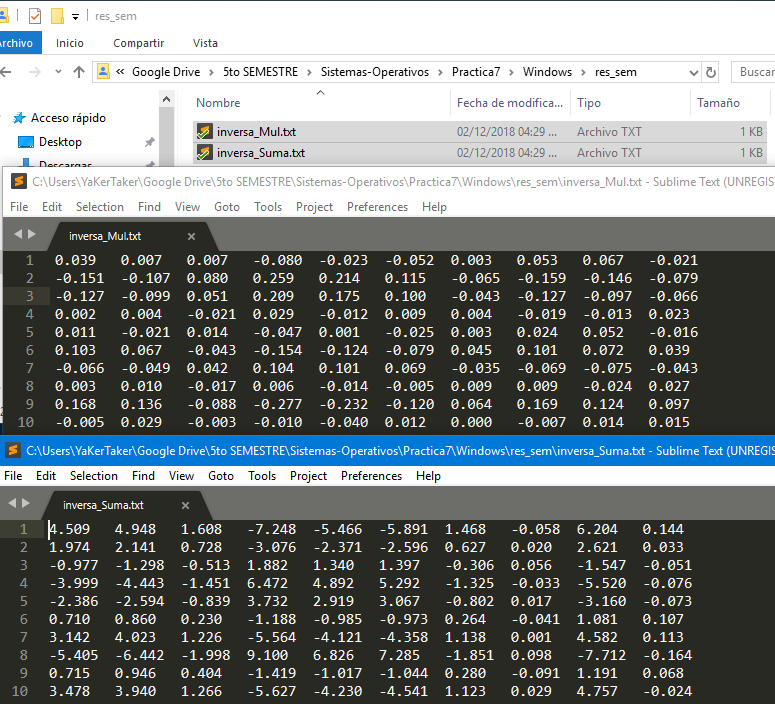
\includegraphics[width=0.82\textwidth]{Practica6/Images/Windows/4/4_5.PNG}
                \end{figure}
                \clearpage
                \begin{figure}[h!]
                        \centering
                    
                   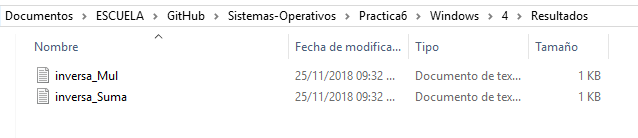
\includegraphics[width=0.91\textwidth]{Practica6/Images/Windows/4/4_6.PNG}
                   
                   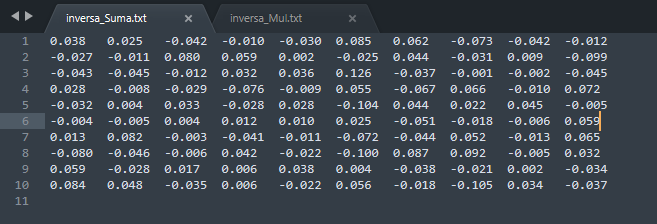
\includegraphics[width=0.91\textwidth]{Practica6/Images/Windows/4/4_7.PNG}
                    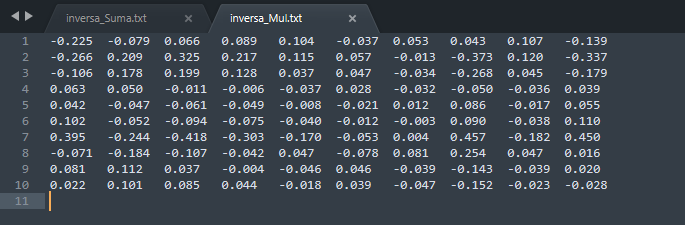
\includegraphics[width=0.91\textwidth]{Practica6/Images/Windows/4/4_8.PNG}
                \end{figure}
                

          \item[\Checkmark] \textbf{Punto 6: Memoria compartida en Windows} 
            \begin{figure}[h!]
                    \centering
                   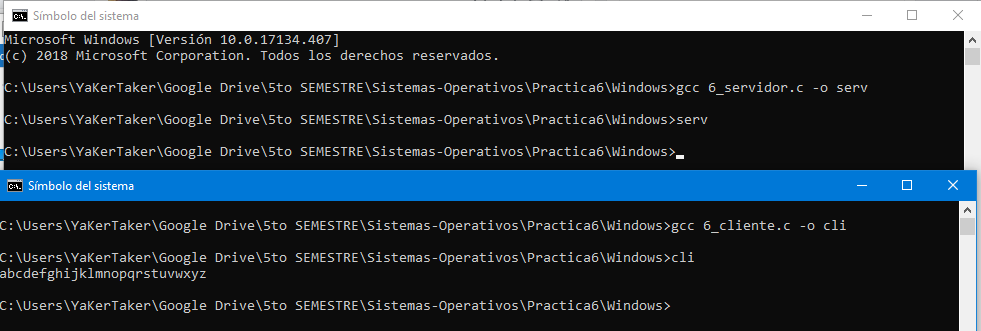
\includegraphics[width=0.91\textwidth]{Practica6/Images/Windows/6.PNG}
            \end{figure}
            \clearpage
            
            \item[\Checkmark] \textbf{Punto 7: Inversa de la suma y multiplicación de matrices con memoria compartida} 
            \begin{figure}[h!]
                    \centering
                     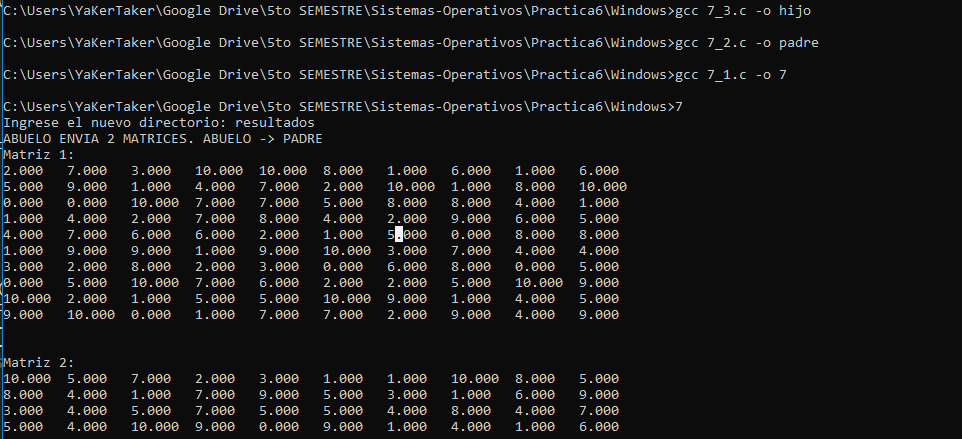
\includegraphics[width=0.9\textwidth]{Practica6/Images/Windows/7_1.PNG}
                   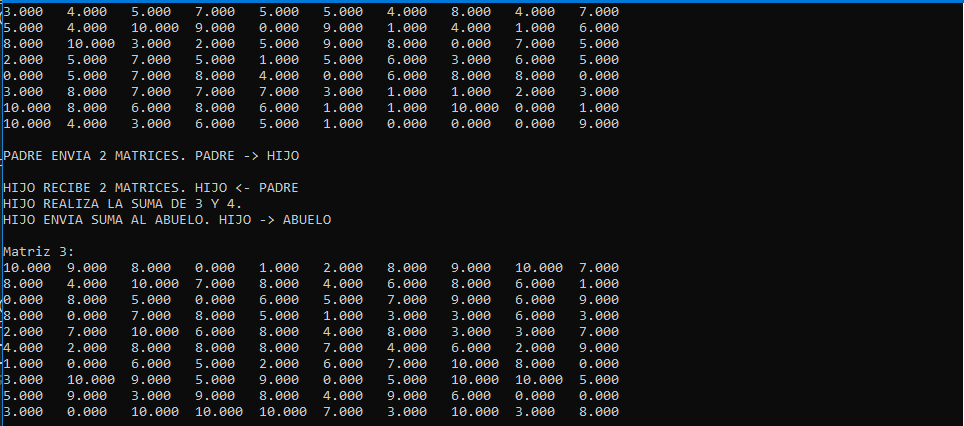
\includegraphics[width=0.9\textwidth]{Practica6/Images/Windows/7_2.PNG}
                   
                   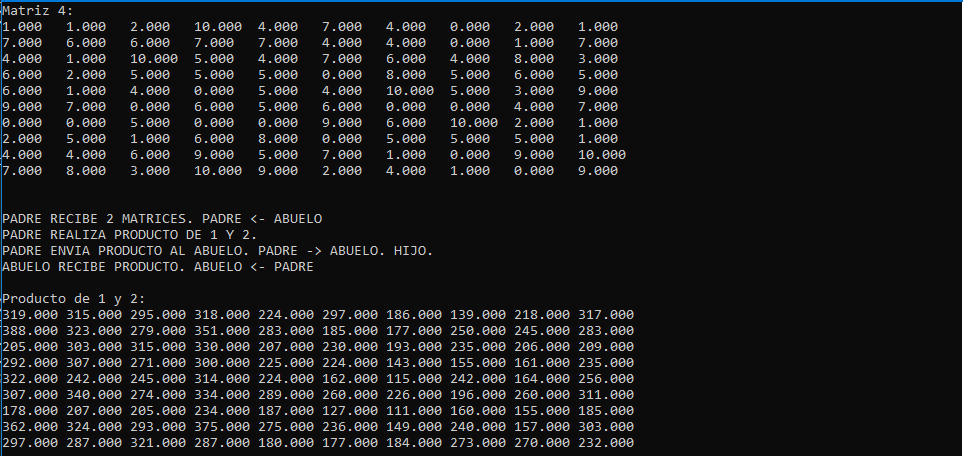
\includegraphics[width=0.9\textwidth]{Practica6/Images/Windows/7_3.PNG}
                   
            \end{figure}
            \begin{figure}[h!]
                    \centering
                     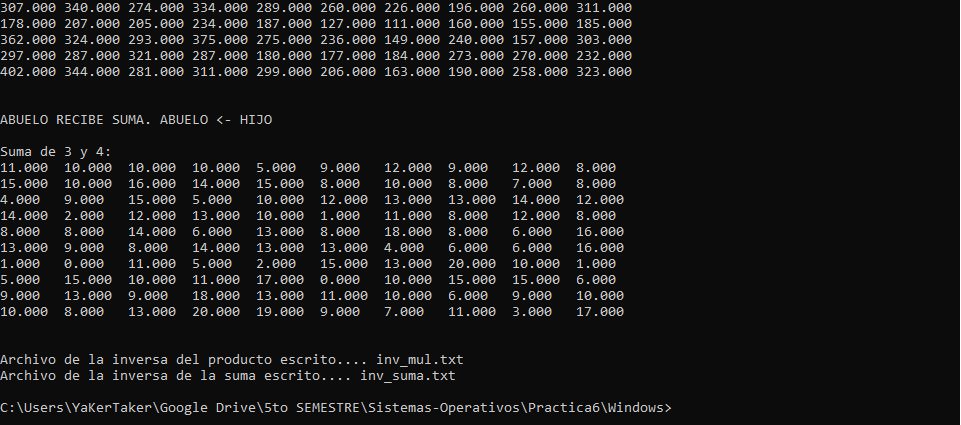
\includegraphics[width=0.9\textwidth]{Practica6/Images/Windows/7_4.PNG}
                   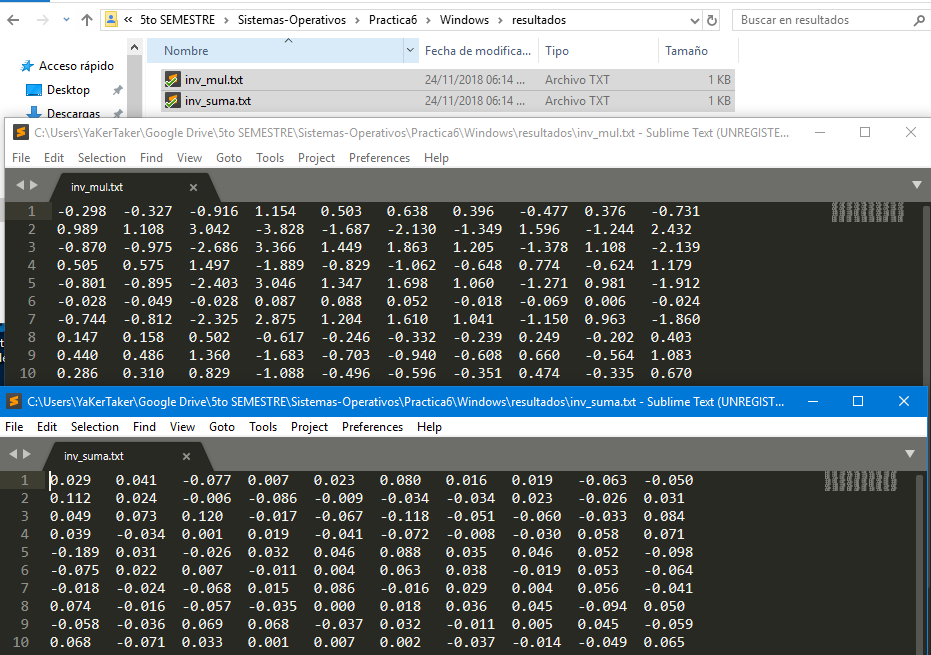
\includegraphics[width=0.9\textwidth]{Practica6/Images/Windows/7_5.PNG}
                   
            \end{figure}
      \end{itemize}


  % /////////////////////////////////////////////////////////////////////////////////////////////////////
  %                                             OBSERVACIONES
  % ////////////////////////////////////////////////////////////////////////////////////////////////////
  
  \section{Observaciones}
  \begin{itemize}
          \item[\Checkmark] En el código de ejemplo 2 de tuberías en Linux, aparece un warning al momento de compilar el programa, esto debido al uso de la función \textbf{gets()}. Sin embargo, la ejecución del programa es la esperada.
          
          \item[\Checkmark] Para ejecutar los códigos de ejemplo de memoria compartida en ambos sistemas operativos, se deben abrir dos terminales, una para el servidor y otra para el cliente. El servidor debe ejecutarse antes que el cliente.
          
          \item[\Checkmark] Para todos los programas, al momento de llenar las matrices con números aleatorios utilizando la función \textbf{rand()}, primero se inicializó el generador \textbf{srand()}, sin embargo, en vez de enviarle como parámetro la clásica función \textit{time(NULL)}, se le envió el número identificador del proceso en donde se encontraba la matriz, esto para evitar que las matrices posean los mismos números aleatorios, debido a la concurrencia en la ejecución de los procesos.
          
          En Linux se envió como parámetro la función \textbf{getpid()}, mientras que en Windows se envió la función \textbf{GetCurrentProcessId()}:
          
          \textbf{srand(getpid())}, \textbf{srand(GetCurrentProcessId())}.
          
           \item[\Checkmark] Para la creación de procesos, en Linux se utilizo la creación por copia de exacta de código, mientras que en Windows la creación por sustitución de código, por eso se crearon varios archivos para un mismo programa.
           
           \item[\Checkmark] Las funciones de operaciones de matrices que se usan en esta práctica, como llenar las matrices con números aleatorios, imprimir las matrices en pantalla, sumar, multiplicar, obtener la inversa y guardar una matriz resultante en un archivo TXT, se encuentran en el archivo llamado \textbf{"funciones.h"}, que ya se explico en prácticas pasadas.
           
           \item[\Checkmark] Para compilar los procesos padre e hijo en los programas de Windows, al inicio del código de cada uno vienen las instrucciones de compilación. Es importante tomar en cuenta esto, debido a que los procesos con mayor jerarquía creados por sustitución de código utilizan rutas o directorios fijos o predeterminados, en donde se encuentran los procesos hijos. En el caso de Linux esto no es necesario.
           
           \item[\Checkmark] En varios programas, tanto en Linux como Windows, surgió el problema de concurrencia entre procesos, pues algunos intentaban a acceder a ciertas variables, por medio de tuberías y memoria dinámica, que aun no se terminaban de calcular. Para solucionar esto, hicimos uso de funciones \textbf{sleep()} para detener por un corto periodo la ejecución de los procesos que deseaban acceder a variables que necesitaban un previo procesamiento.
           
           \item[\Checkmark] En el programa 4 de Linux de tuberías, para enviar y recibir los datos por medio de tuberías utilizando las funciones \textbf{read()} y \textbf{write()}, se necesito de dos ciclos anidados para ir mandando posición por posición, de manera individual para evitar errores. En este mismo programa, la creación de procesos se hizo de forma inversa a como la veníamos manejando, trabajando primero sobre el proceso padre y luego sobre los hijos.
           
            \item[\Checkmark] En el programa 4 de Windows de tuberías, en los resultados se van mostrando, imprimimos cuando llega al PADRE, eso se hace para que notemos que el programa esta funcionando de manera correcta y que las tuberías están funcionando. Por lo anterior, se ven comentarios que muestran como funciona el programa, estos sirven para identificar como interactúan.
          
\end{itemize}


  % ////////////////////////////////////////////////////////////////////////////////////////////////////
  %                                          ANALISIS CRITICO
  % ////////////////////////////////////////////////////////////////////////////////////////////////////
  
  \section{Análisis Crítico}
  
  Nuevamente nos valemos de llamadas al sistema para la creación de tuberías y memoria compartida.
  
  En Linux tenemos lo siguiente
  \begin{multicols}{2}
      \textbf{Tuberías}:  
      \begin{itemize}
          \item[\Checkmark] Crear una tubería con pipe().
          \item[\Checkmark] Escribir datos con Write().
          \item[\Checkmark] Leer datos con read().
      \end{itemize}
\columnbreak
        \textbf{Memoria compartida}:  
      \begin{itemize}
          \item[\Checkmark] Obtiene el identificador con shmget().
          \item[\Checkmark] Adjunta identificador con shmat().
      \end{itemize}
  \end{multicols}

  En Windows tenemos lo siguiente
    \textbf{Tuberías}:
    \begin{itemize}
        \item[\Checkmark] Crear una tubería con CreatePipe().
        \item[\Checkmark] Escribir datos con WriteFile().
        \item[\Checkmark] Leer datos con ReadFile().
    \end{itemize}

    Recordando la información que el profesor nos dio en la clase, se mencionaba que en el caso de las tuberías el Sistema operativo trabaja la información como archivos, la razón es porque las variables e incluso apuntadores no se permiten compartir entre procesos.
    
    Otra característica que se vio en el desarrollo de esta práctica, es que las tuberías no son bidireccionales, eso se nota porque para enviar una matriz se usa una tubería y para recibirla otra.
    
    Podemos decir que en el sistema operativo Windows se muestra casi la misma versatilidad en tuberías y memoria compartida que en Linux, pero este eleva su complejidad de uso.
    
    
  % ///////////////////////////////////////////////////////////////////////////////////////////////////
  %                                            CONCLUSIONES
  % ///////////////////////////////////////////////////////////////////////////////////////////////////
  
  \section{Conclusiones}
    La memoria compartida y las tuberías son de gran ayuda para compartir información entre distintos procesos, pero cada uno de estos mecanismos aporta diferentes características, debido a su forma de operar, por lo tanto, se debe conocer adecuadamente su sintaxis y funcionamiento para poder aprovechar sus funcionalidades. Las tuberías pueden enviar información a procesos hijos, pero estas son únicamente unidireccionales, por lo que es necesario crear una para cada comunicación entre ellos, es decir, de ida como de vuelta. Por otro lado, la memoria compartida proporciona más posibilidades, ya que su funcionamiento es similar a la memoria dinámica,se asigna a un apuntador para acceder a ella mediante la llave, la cual sirve para localizarla y acceder, teniendo menos restricciones que las tuberías.

\end{document}